\clearpage
\sffamily
{\bfseries\color[rgb]{0.4,0.4,0.4}
Part A: Push Recovery }

\bigskip

The goal of the push recovery challenge is to withstand a strong push. PET bottles, partially filled with sand or water to determine the weight, cushioned with a layer of foam material (max. 1 cm thick), and suspended by a rope, will be used as a pendulum to apply the push. A 1 kg weight will be used for KidSize, 2 kg for TeenSize, and 3 kg for AdultSize. 

The length of the rope (between 1 and 2 meters) will remain fixed for all trials in a size class. The rope is attached to a frame with variable height, which is used to adjust the bottom of the bottle to be at the height of the center of mass of the robot. To swing the bottle against the robot's body, the pendulum is released from an angle which is measured by the ground projected distance between the robot and the bottle. At each attempt, the team announces the ground projection distance for the pendulum. The robot \textcolor{magenta}{must be walking in place during the attempt}. A push is successfully absorbed when after receiving the push, the robot returns to a stable standing or walking posture. 

\textcolor{magenta}{A trial consists of three random pushes. For a fully successful trial, the robot needs to accomplish the push recovery for three out of three pushes. For a partially successful trial, the robot needs to accomplish the push recovery for two out of three pushes.} The robots are first ranked by the \textcolor{magenta}{square root of the linear momentum $H = L - \sqrt{L^{2} - D^{2}}$ divided by the robot weight} for fully successful trials and then for partially successful trials. The formula for calculating the rank is thereby:

\begin{align*}
\dfrac{\sqrt{H}}{m_{Robot}} =  \dfrac{\sqrt{L - \sqrt{L^{2} - D^{2}}}}{m_{Robot}}
\end{align*}

\begin{figure}[h]
\begin{center}
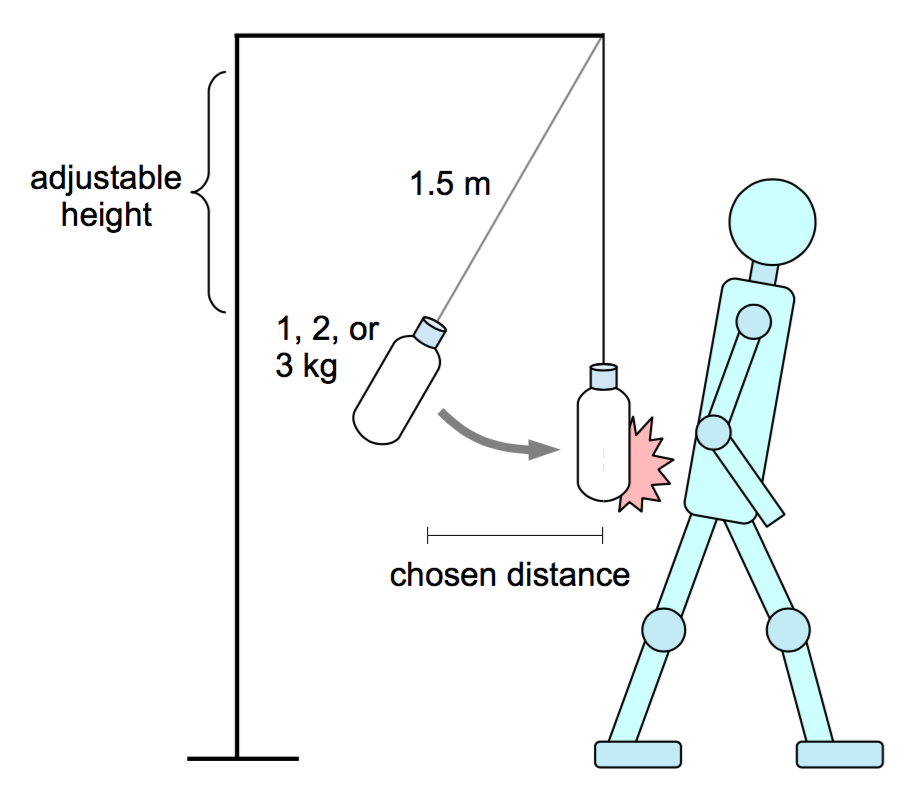
\includegraphics[scale=1.0]{img/push_recovery.png}
\caption{Setup for the push recovery challenge. }
\end{center}
\end{figure}